\chapter{Implementering}

\section{Fugt- og temperatursensor (LB)}
Implementeringen af sht21p er sket ved at designe et print som indeholder sht21p og et 2. ordensfilter. 
Da sht21p-komponentet er et SMD-komponent var det ikke muligt at opstille kredsløbet på vero-board. Det var derfor nødvendigt at få et print produceret. Til design af printet blev CadSoft EAGLE PCB design software brugt. Nedenfor ses diagram og PCB layout af printet.


\begin{figure}[htb]
\centering
{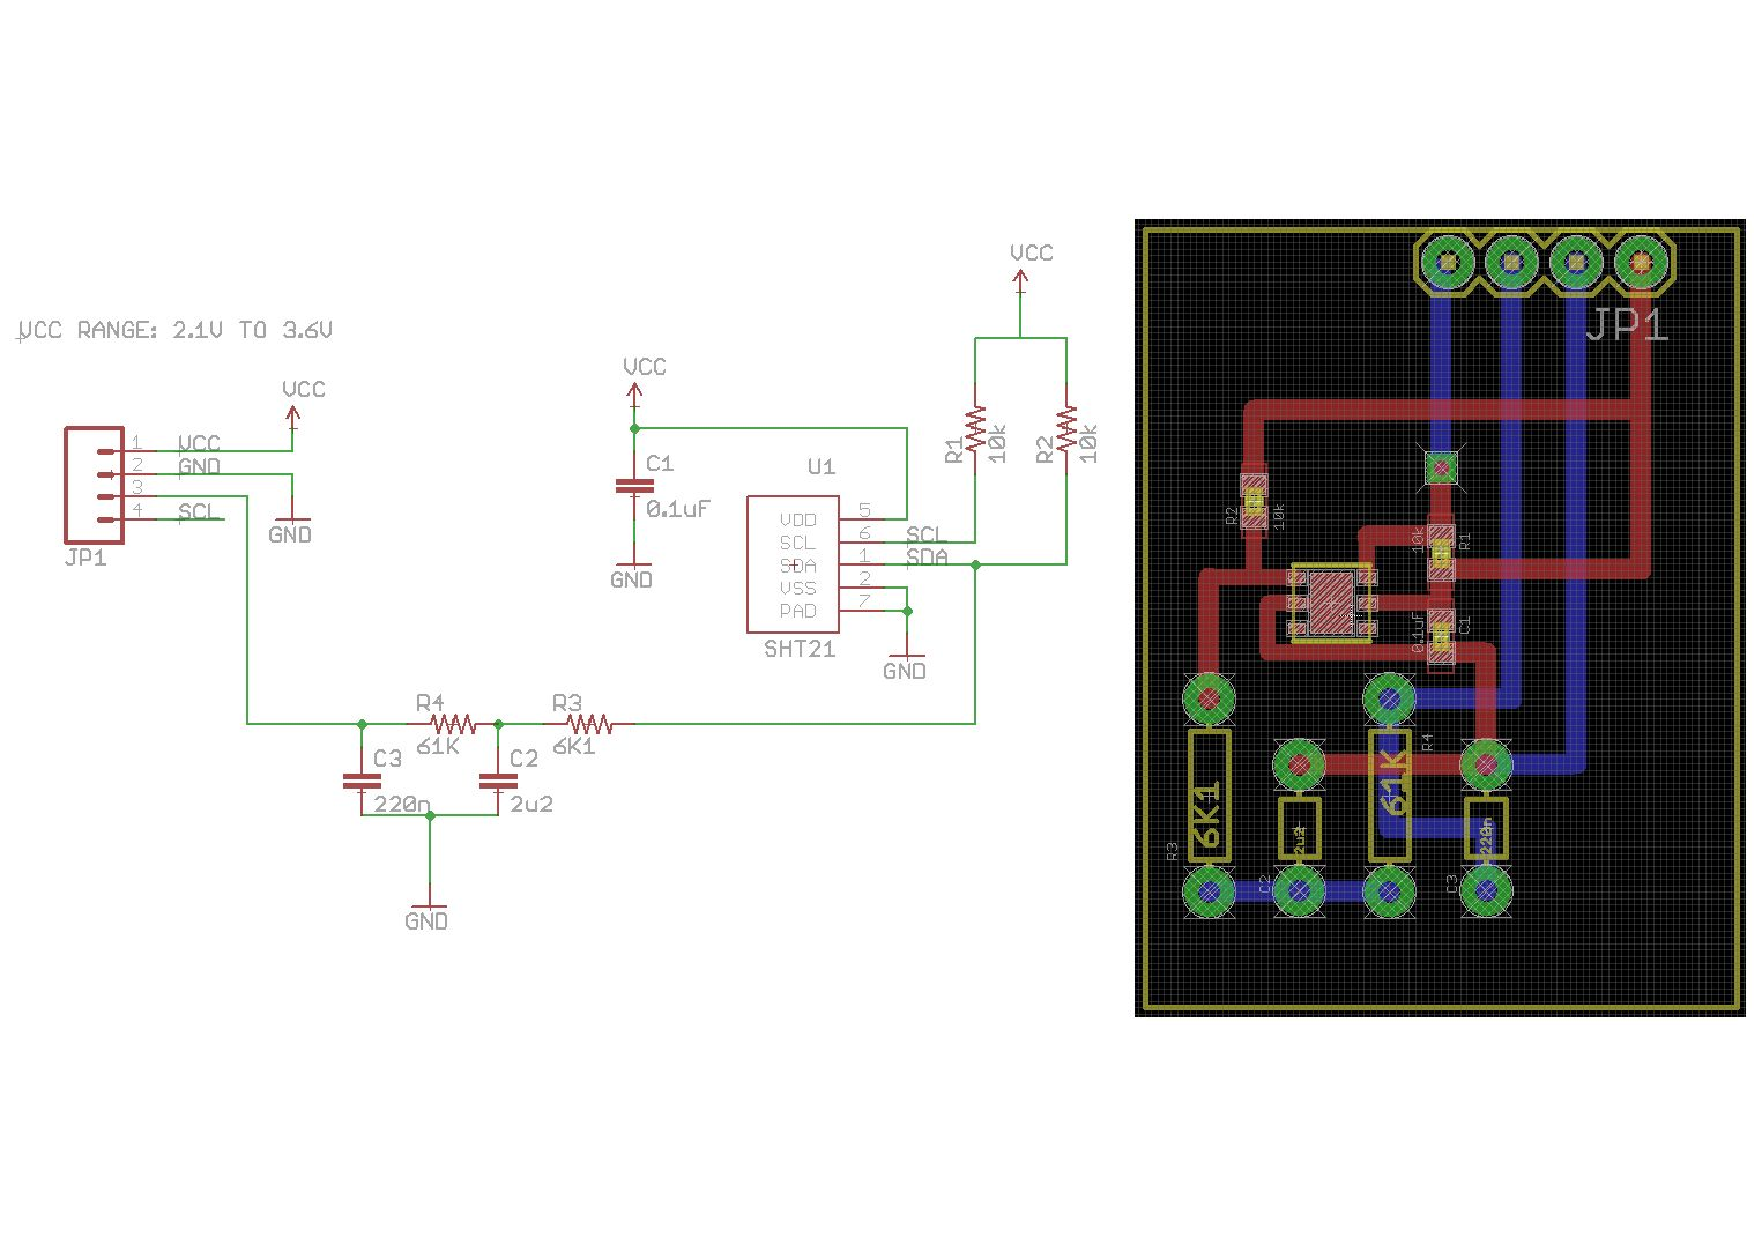
\includegraphics[width=\textwidth]{filer/implementering/SHT21P-pcb-sch}}
\caption{Schematic og layout af SHT21P kredsl\o{}b}
\label{lab:SHT21P-kredsloeb}
\end{figure}

Kredsløbet på figur \ref{lab:SHT21P-kredsloeb} blev eksporteret til gerberfiler og sendt til elektronikværkstedet som så ætsede printet og derefter monteret op.



\section{Tilslutningsprint (SK)}
Implementeringen af tilslutningsprintet er lavet ved at konstruere et veroboard print. Tilslutningsmulighederne på printet består af en indgang til 12 VDC fra PSUen, en USB-udgang der forsyner Enheden, 12 harwinstik til de forskellige sensorer og en udgang der styrer sprinklerrelæet. På figur \ref{lab:Tilslutningsprint} kan det færdige resultat ses. 

\begin{figure}[htb]
\centering
{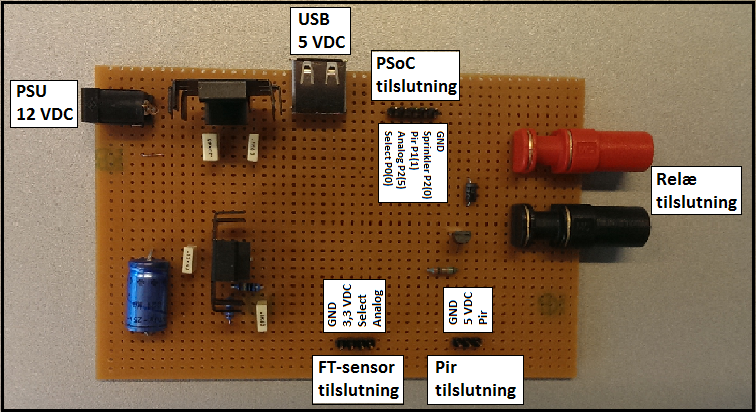
\includegraphics[width=0.70\textwidth]{filer/pics/Tilslutningsprint}}
\caption{Tilslutningsprint til forbindelse af sensorer og PSoC4}
\label{lab:Tilslutningsprint}
\end{figure}




\section{FT-Sensor og sprinkler API (JS)}
%% psoc_api

API til styring af PSoC, herunder sensor og sprinkler, er implementeret i PSoC Creator. Top designet består af en ADC\_SAR\_Seq, en analog pin og to digitale pins til at styre henholdsvis sprinkler og Select til bestemmelse af temperatur- eller fugtighedsdata for SHT21p.
I top designet er der angivet følgende pins. ''P\_FT1'', ''P\_FT2'', ''P\_VP'' disse forbindes til henholdsvis pin P2[5], P0[0] og P2[0]. P\_FT1 oprettes som en analog pin og de to andre som digitale output pins. Under konfiguration for de digitale pins fravælges ''HW Connection'' under Digital Output. For nærmere opsætning af pins henvises til figur \ref{lab:P_PV_config} og figur \ref{lab:P_FT2_config}

\begin{figure}[htb]
\centering
{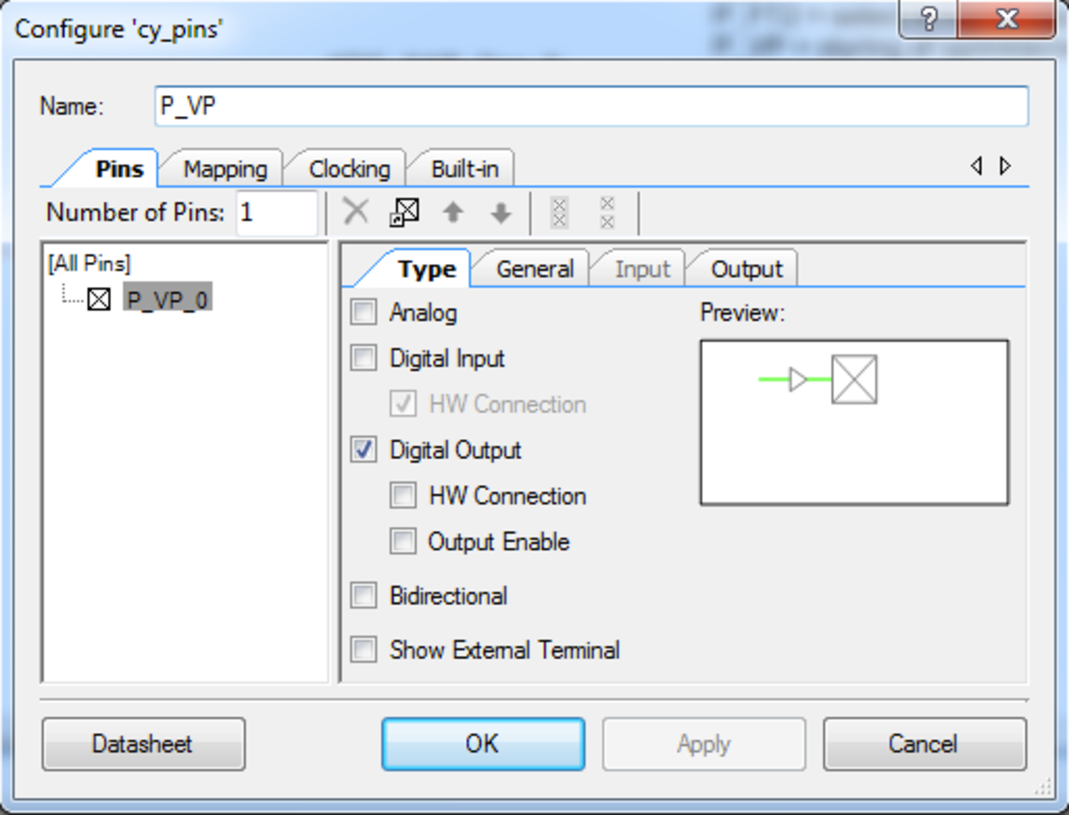
\includegraphics[width=0.70\textwidth]{filer/pics/P_PV_config}}
\caption{Konfiguration for P\_PV}
\label{lab:P_PV_config}
\end{figure}


\begin{figure}[htb]
\centering
{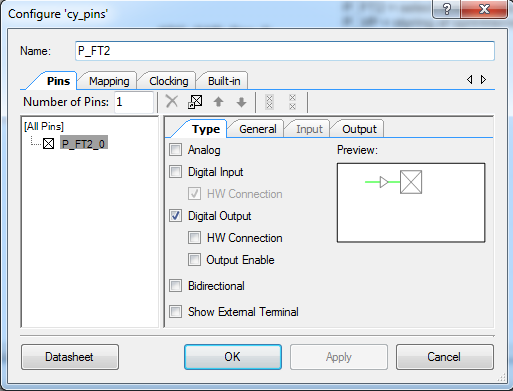
\includegraphics[width=0.70\textwidth]{filer/pics/P_FT2_config}}
\caption{Konfiguration for P\_FT2}
\label{lab:P_FT2_config}
\end{figure}  

Under konfiguration for ADC-komponenten vælges Vref til VDDA og Single ended negative input vælges til Vss. Dette sætter ADCen op til at bruge 0 V som referencespænding.

Da PSoC kun har en SAR komponent er det nødvendigt at initialisere denne i sensorPackage-driveren.

\begin{figure}[htb]
\centering
{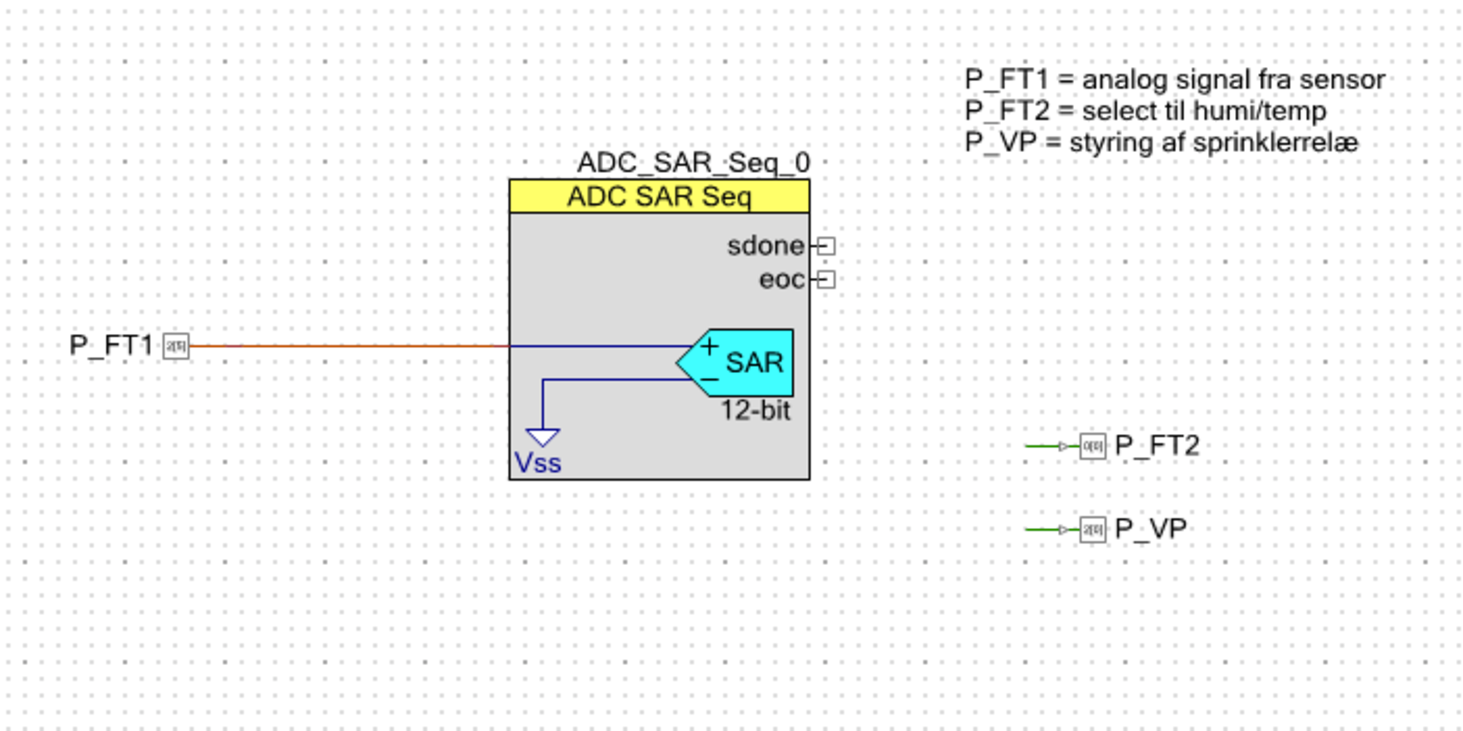
\includegraphics[width=0.70\textwidth]{filer/pics/psoc_api_topdesign}}
\caption{Top Design for PSoC API}
\label{lab:psoc_api_topdesign}
\end{figure}

\begin{figure}[htb]
\centering
{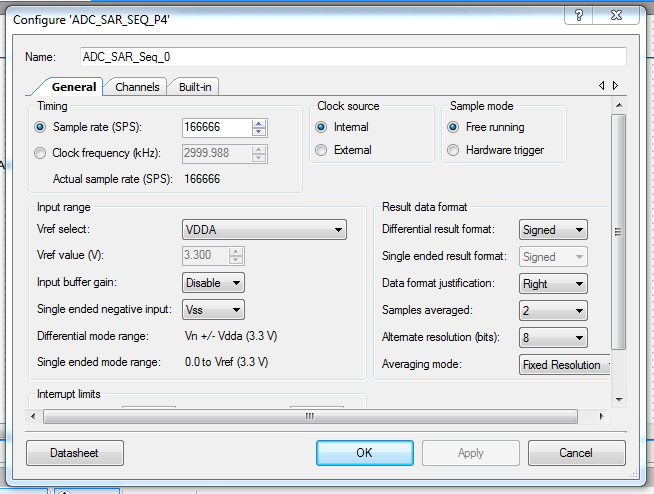
\includegraphics[width=0.70\textwidth]{filer/pics/psoc_api_config1}}
\caption{Konfiguration af Vref og Single ended negative input}
\label{lab:psoc_api_config1}
\end{figure}

\begin{figure}[htb]
\centering
{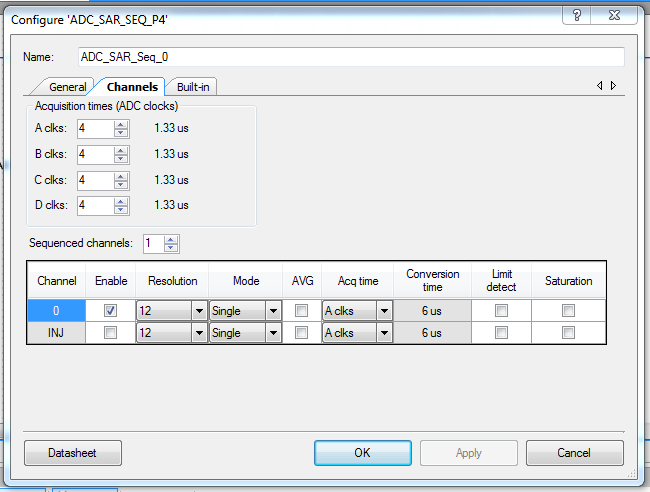
\includegraphics[width=0.70\textwidth]{filer/pics/psoc_api_config2}}
\caption{Konfiguration af Channels for ADC}
\label{lab:psoc_api_config2}
\end{figure}

\section{230 V / 5 V relæ (PO)}
% 230V Relæ

Relæet er implementeret som beskrevet i designdelen. Figur \ref{lab:Relay_inside} viser relæet som det er implementeret. Relæet er indbygget i en lukket kasse med transparent låg. 
Veroboard er benyttet som sokkel for relæet. Installationsledning er benyttet til 230V spændingen 0,75 kvadrat.
Den lyseblå leder er nul og den sorte leder er 230V fasen 
Jord/beskyttelseslederen er den gul/grønne, denne går direkte fra indgang (apparatstik) til udgang (230V stikkontakt). 
  


\begin{figure}[htb]
\centering
{\includegraphics[width=0.60\textwidth]{filer/implementering/relay_inside}}
\caption{Relæet uden påmonteret låg}
\label{lab:Relay_inside}
\end{figure}

Figur \ref{lab:Relay_connection} viser relæet fra begge ender. Veste side viser indgangen, som består af ét 230V apparatstik og 2 bananstik. Apparatstikket tilsluttes en stikkontakt som er tændt. Bananstikkene tilsluttes tilslutningsprintet. Højre side viser 230V stikkontakten som tændes/slukkes af relæet. Vandpumpen tilsluttes denne stikkontakt.

\begin{figure}[htb]
\centering
{\includegraphics[width=0.80\textwidth]{filer/implementering/relay_connection}}
\caption{Relæet set fra begge ender.}
\label{lab:Relay_connection}
\end{figure}

Relæet er godkendt af Torben Lund Jensen fra værkstedet på IHA.

\section{Sprinkler og Alpha 2 pumpe (PO)}
% Vandpumpe implementering 

\textbf{Sprinkler} \newline
Sprinkleren kræver et 1/2" gevinds tilslutning. Dette løses vha. en konisk fitting, som har et udvendigt 1/2" gevind i den ene ende og en konisk slangetilslutning i den anden. En alm. husholdningsvandslange sættes på slangetilslutningen med et spændebånd. 

\textbf{Alpha 2 pumpe}  \newline
Alpha 2 pumpens tilslutning er 2" udvendigt gevind. Grundet økonomiske omstændigheder er en hjemmelavet tilslutningsløsning valgt. En drejebænk er benyttet til at dreje 2" forskruninger der ender ud i konisk slangetilslutning. Det drejes i alt 2 stk. Disse slangetilslutninger passer til husholdningsvandslangn og forbindes herved til vandtilførsel og sprinkler.

Figur \ref{lab:fitting_alpha2} viser en af de færdige studser til alpha 2 pumpen. 

\begin{figure}[htb]
\centering
{\includegraphics[width=0.60\textwidth]{filer/implementering/studs_alpha2}}
\caption{Studs til Alpha 2 pumpen}
\label{lab:fitting_alpha2}
\end{figure}



\newpage
\section{SPI (MK PO)}
% SPI API


% Indledning 

SPI kommunikationen har en API klasse på Master skrevet i \verb+C+++ og en handler på Enhed skrevet i \verb+C+.

For at add-on printet på Devkit8000 kan bruge GPIO benene til SPI kommunikationen er det nødvendigt at rute dem korrekt, dette gøre ved at bruge følgende 2 kommandoer.

\begin{itemize}
\item \verb+echo 0x3 > /sys/class/cplddrv/cpld/spi_route_reg+
\item \verb+echo 0x1 > /sys/class/cplddrv/cpld/ext_serial_if_route_reg+
\end{itemize}

Kernemodulet skal også indsættes og oprette en system node, i APIen bruges \verb+/dev/spi_dev+ så denne er fast.
Alt dette er skrevet i et shell script der håndtere alt indsætning og oprettelse af kernefilen, se bilag \verb+insert_SPI_dev.sh+

% SPI API

\subsection{SPI API}
% SPI API

SPI\_api er en klasse til at styre SPI kommunikationen. Den består af en række metoder beskrevet i afsnit \ref{fig:SPI API klassediagram}.

Alle metoderne er stort set opbygget ens.

\subsubsection*{Open}

De har alle en \verb+open()+ metode der sørger for at åbne system filen der enten skal skrives til eller læses fra. Hvis der sker en fejl i open, returnere den så en passende negativ fejl, i dette tilfælde fejlen LOG\_ERR.

\begin{lstlisting}[language=C]
/* Open file */
fp = open("/dev/spi_dev", O_RDWR);
if(fp < 0){
	printf("OPEN ERROR: %d\n", fp);
	close(fp);
	return -LOG_ERR;
}
\end{lstlisting}

\subsubsection*{Close}

Der er også altid en \verb+close()+ metode, der sørger for at lukke den åbnede fil ned igen. Denne metode er også lagt i alt fejlhåndtering, for at undgå systemfejl på Masteren, hvis der skulle ske fejl.



\begin{lstlisting}[language=C]
/* Close file */
close(fp);
\end{lstlisting}

\subsubsection*{Write \& Read}

Ind i mellem disse er så en \verb+write()+ eller/og en \verb+read()+ metode, der sørger for at der bliver læst fra eller skrevet til Enheden via SPI. Her er nogle eksempler på metoderne.

\verb+Write()+ metoden bruges i starten af alle metoder til at vælge hvad der skal ske på Enheden ved at skrive en char kommando til den. Den bruges også, som her, til at skrive parametrene temp og humi til Enheden. Her modtages parametrene som floats, konverteres til chars og skrives enkeltvis til Enheden med en for-løkke.

\begin{lstlisting}[language=C]
int SPI_api::config(int unit, float temp, float humi)
{
char tempArray[6];	// T T T . T \0
char humiArray[4];	// F F F \0

/* Parse floats to CharArrays */
snprintf(tempArray, sizeof(tempArray), "%05.1f", temp);
snprintf(humiArray, sizeof(humiArray), "%03.0f", humi);
..
..
..
/* Write temp to target without 0-termination */
for(int i = 0 ; i < 5 ; i++){
	err = write(fp, &tempArray[i], dataLen);
		if(err < 0){
		printf("WRITE ERROR: %d\n", err);
		close(fp);
		return -CONF_ERR;
	}
}

/* Write humidity to target without 0-termination */	
for(int i = 0 ; i < 3 ; i++){		
	err = write(fp, &humiArray[i], dataLen);
	if(err < 0){
		printf("WRITE ERROR: %d\n", err);
		close(fp);
		return -CONF_ERR;
	}
}
..
..
}
\end{lstlisting}

\verb+Read()+ metoden modtager chars fra Enheden og behandler dem. I koden nedenfor ses implementeringen for \verb+getLog()+ metoden som læser på en buffer på Enheden hvori der ligger Data og Fejl. Disse chars bliver så lagt i en vector<string> så programmet på Masteren har en nem måde at håndtere fejl og log-data på. Vector og alle string variablerne nulstilles med \verb+clear()+ for en god ordens skyld, da der nødigt skulle stå noget forkert i dem inden de pushes med ny data.

Den første \verb+read()+ metode man støder på, læser bufferlængden fra Enheden, som der sørger for der ikke læses på noget data der ikke er tilstede, senere i metoden.

Så er der en for-løkke der starter med at kigge på om der er et 'D' for data eller 'E' for fejl. Disse laver hhv. 10 og 3 læsninger, som der bygges en string af, der pushes til en vector. Hvis der kommer et 'D' ligges det på den første plads i en string sammen med de næste 10 læsninger. Dette er tilsvarende ved en fejl, dog kun med 3 læsninger efter det læste 'E'.

\begin{lstlisting}[language=C]
int SPI_api::getLog(vector<string> &data, int * units, int size)
{
..
..
..
char charArrayLen;		// Variable for charArray size from target
char charResult;		// Used for buffering read chars
string stringResult;
	stringResult.clear();
string stringDataResult;
	stringDataResult.clear();
string stringErrorResult;
	stringErrorResult.clear();
vector<string> vectorResult;
	vectorResult.clear();
..
..
..

/* Read charArray length from target */
err = read(fp, &charArrayLen, dataLen);
if(err < 0){
	printf("READ ERROR: %d\n", err);
	close(fp);
	return -LOG_ERR;
}
	
/* Vector Builder looking for D's or E's */
for(i = 1 ; i < charArrayLen ; i++){
	err = read(fp, &charResult, dataLen);
	if(err < 0){
		printf("READ ERROR: %d\n", err);
		close(fp);
		return -LOG_ERR;
	}

	if(charResult == 'D'){
		stringDataResult.push_back(charResult); // Push 'D' to stringDataResult
		
		// Build rest of stringDataResult
		for(int c = 0 ; c < dataStringLen ; c++){
			err = read(fp, &charResult, dataLen);
			if(err < 0){
				printf("READ ERROR: %d\n", err);
				close(fp);
				return -LOG_ERR;
			}			
			stringDataResult.push_back(charResult);
			
			// Error handling, prevent to read on non-existing data
			if(i >= (charArrayLen-1)){
				printf("Error in buffer from unit\n");
				return -LOG_ERR;
			}
			i++;	// Increment 1st for-loop counter
		}
		
		// Push string to vectorResult
		vectorResult.push_back(stringDataResult);
		stringDataResult.clear();
	}
	
	if(charResult == 'E'){
		stringErrorResult.push_back(charResult); // Push 'E' to stringErrorResult
		
		// Build rest of stringErrorResult
		for(int c = 0 ; c < errorStringLen ; c++){
			err = read(fp, &charResult, dataLen);
			if(err < 0){
				printf("READ ERROR: %d\n", err);
				close(fp);
				return -LOG_ERR;
			}
			stringErrorResult.push_back(charResult);

			// Error handling, prevent to read on non-existing data
			if(i >= (charArrayLen-1)){
				printf("Error in buffer from unit\n");
				return -LOG_ERR;
			}
				i++;	// Increment 1st for-loop counter
		}

		// Push string to vectorResult and clear string
		vectorResult.push_back(stringErrorResult);
		stringErrorResult.clear();
	}
}
\end{lstlisting}

\subsubsection*{Clear buffer}

Alle metoderne har også en Clear buffer funktion. Denne benytter \verb+write()+ metoden, til at skrive et 'C' til Enheden for at nulstille tx-bufferen. Den bruges også for at tilgå switchen for alle write-only metoderne.

\begin{lstlisting}[language=C]
/* Clear buffer */
err = write(fp, &CL_BUF, 1);
if(err < 0){
	printf("CLEAR ERROR: %d\n", err);
	close(fp);
	return -CONF_ERR;
}
\end{lstlisting}

Resten af implementeringen findes i bilag.


% SPI HANDLER

\subsection{SPI Handler}
% SPI Handler

\subsubsection*{Top-design - PSoC Creator 3.0}

Topdesignet (figur\ref{lab:topdesign_spi}( består af en SPI blok, samt 3 digitale output pins. Herunder beskrives hvordan elementerne i topdesignet skal indstilles.

\begin{figure}[H] \centering
{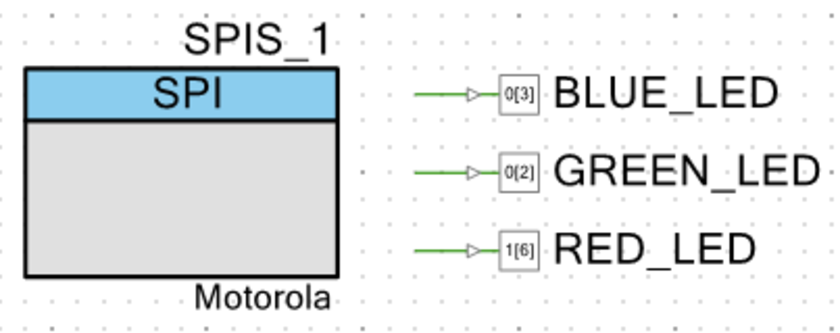
\includegraphics[width=0.4\textwidth]{filer/implementering/spi/spi_handler_topdesign}}
\caption{Topdesign for SPI og led}
\label{lab:topdesign_spi}
\raggedright
\end{figure}

Basis indstillingerne for SPI blokken ses i figur \ref{lab:spi_basic_config}. Mode sættes til slave, og SCLK mode sættes til CPOL=0, CPHA=0.

\begin{figure}[H] \centering
{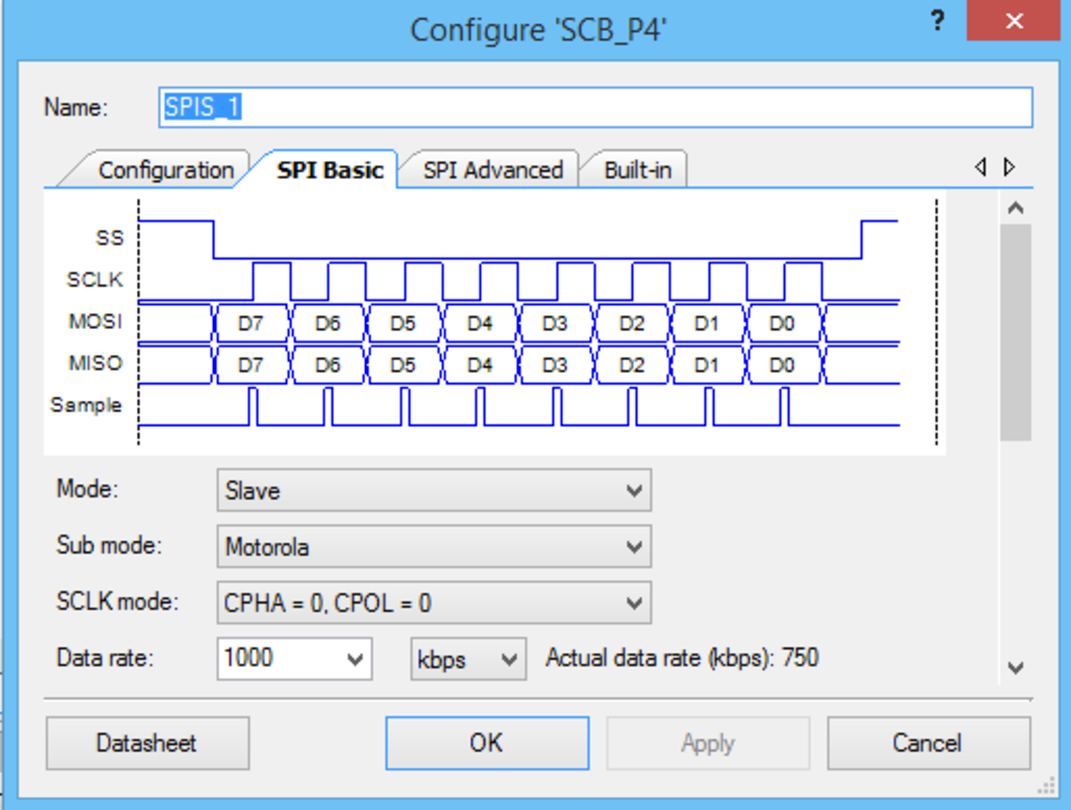
\includegraphics[width=0.8\textwidth]{filer/implementering/spi/spi_handler_topdesign_spi_basic}}
\caption{Konfigurering af SPI (SPI basic)}
\label{lab:spi_basic_config}
\raggedright
\end{figure}

De avancerede indstillinger for SPI blokken ses i figur \ref{lab:spi_advanced_config}. Buffer size sættes til 8 bit for både RX og TX. Interruptet sættes til internt og interrupt kilden er RX FIFO not empty og RX FIFO full.

\begin{figure}[H] \centering
{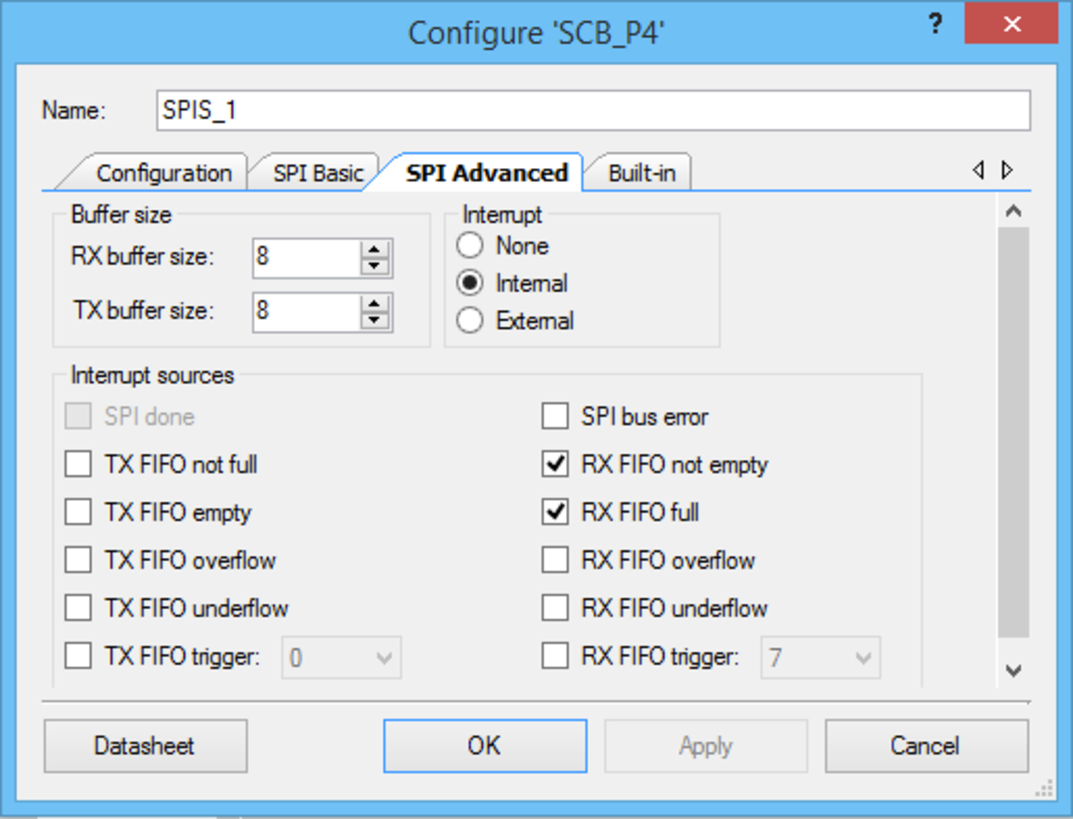
\includegraphics[width=0.8\textwidth]{filer/implementering/spi/spi_handler_topdesign_spi_advanced}}
\caption{Konfigurering af SPI (SPI advanced)}
\label{lab:spi_advanced_config}
\raggedright
\end{figure}

De 3 output pins (GREEN\_LED, BLUE\_LED, RED\_LED) skal sættes til digital output uden hardware connection.
Figur \ref{lab:led_pins_config} viser hvordan indstillingen skal være, dette er gældende for alle 3 pins. 

\begin{figure}[H] \centering
{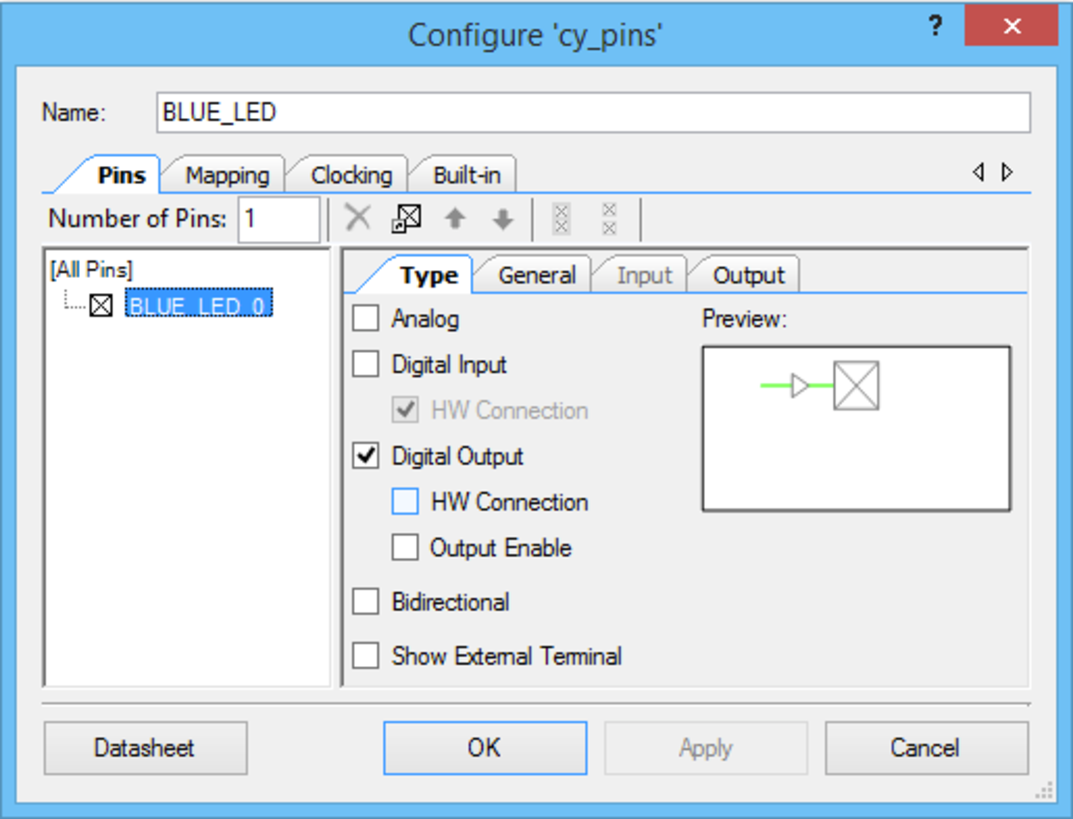
\includegraphics[width=0.8\textwidth]{filer/implementering/spi/spi_handler_topdesign_led}}
\caption{Konfigurering af pins}
\label{lab:led_pins_config}
\raggedright
\end{figure}


\subsubsection*{ISR}

SPI handleren består stort set kun af én interrupt rutine. Der tages udgangspunkt i de vigtige dele af rutinen. Og resten af koden kan ses i bilag.

Selve interrupt-rutinen er bygget op med en switch, der vælger en case alt efter input fra Masteren. Der tilgås kun switchen hvis der kommer en kommando der skal svare tilbage til Master (\verb+'R','L','V'+) eller en Clear buffer kommando \verb+'C'+, derefter kigges der på plads [0] i spiBuffer arrayet, og handles alt efter hvad der står der. Dvs. hvis Enheden skal aktiveres, sendes først et \verb+'A'+ fra Master som læses ind i spiBuffer[] arrayet efterfulgt af et \verb+'C'+ som tilgår switchen.
 
\begin{lstlisting}[language=C]
char spiBuffer[64];
..
..
..
CY_ISR(isr_spi_rx) {

	char cmd = '0';
	..
	.. 
	cmd = SPIS_1_SpiUartReadRxData(); 
    
    spiBuffer[spiCounter] = cmd;
    spiCounter++;
..
..
    if ((cmd == 'R') || (cmd == 'C') || (cmd == 'L') || (cmd == 'V')){
    	switch (spiBuffer[0]) {
\end{lstlisting}

Alle kommandoer der kræver et svar tilbage på SPI, bruger \verb+'R'+ casen, men eftersom PSoC4 kræver noget tid til at hente og skrive i tx-bufferen er koden lavet sådan at man er på forkant med en læsning. Dvs. når der laves en læsning \verb+'R'+ fra Masteren, er der allerede skrevet til tx-bufferen, så man reelt læser data ud med det samme. 

Det er derfor switchen tilgåes ved alle ''Read'' kommandoer, så hvor der f.eks. skal verificeres, laves der en læsning af Enhedens enhedsnummer. I eksemplet nedenfor er en global char brugt som enhedsnummer, denne læses ind i tx-bufferen når case \verb+'V'+ køres. Og når så case \verb+'R'+ køres, læses unitNo variablen først, hvorefter der skrives en ny værdi ind i tx-bufferen til næste \verb+'R'+ køres.

\begin{lstlisting}[language=C]
char unitNo = '1';
int spiCounter = 0;
int spiReadCounter = 0;
..
..
..
CY_ISR(isr_spi_rx) {
..
..
..
    		case 'V':
					..
					..
					..
                    SPIS_1_SpiUartClearTxBuffer();
                    SPIS_1_SpiUartWriteTxData(unitNo);
                    spiCounter = 0;
    			break;
..
..
..
            case 'R':
                    SPIS_1_SpiUartClearTxBuffer();
                    SPIS_1_SpiUartWriteTxData(spiTxBuffer[spiReadCounter]);
                    spiCounter = 0;
                    spiReadCounter++;
                break;
\end{lstlisting}




\section{PIR API (SK MK)}
%pir api
Pir API'en er implementeret i PSoC creator. Top designet består af en input pin (P1[1]) der modtager et signal fra pir-sensoren når der er bevægelse, se figur \ref{lab:pir_topdesign}. På figur \ref{lab:pir_topdesign_1} og \ref{lab:pir_topdesign_2} ses opsætningen af P-PIR, den har en HW connection til isr-pir og er indstillet til at have en pulldown modstand for at sikre at der står lav på pinen når der ikke er signal. Denne pin går ind og aktiverer en ISR routine. I source filen ses det at selve ISR funktionen går ind og kalder en metode fra controlleren, der deaktivere sprinkleren og starter en timer på 30 min før der igen kan vandes.   

\begin{figure}[htb]
\centering
{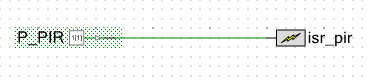
\includegraphics[width=0.60\textwidth]{filer/pics/pir_api_topdesign}}
\caption{Top Design for pir API}
\label{lab:pir_topdesign}
\end{figure}

\begin{figure}[htb]
\centering
{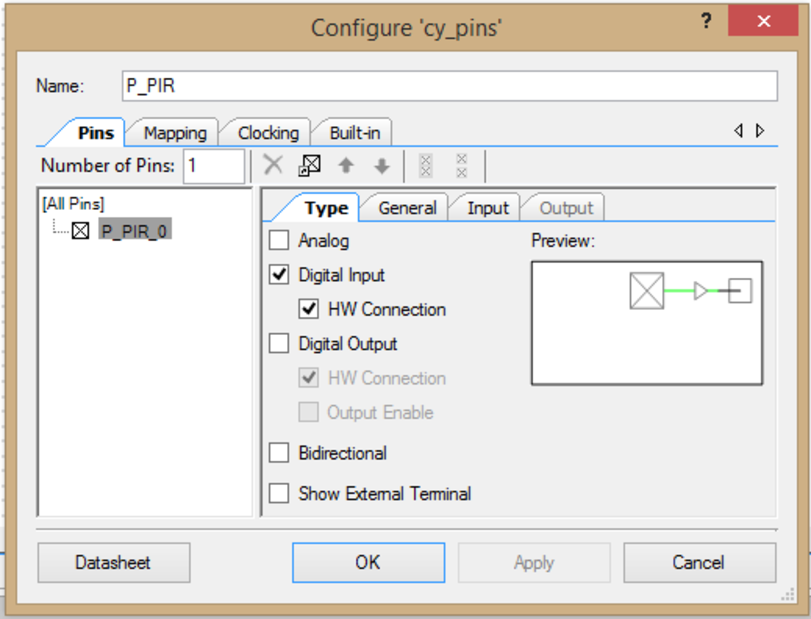
\includegraphics[width=0.60\textwidth]{filer/pics/pir_api_topdesign_1}}
\caption{Konfiguration af pir pin}
\label{lab:pir_topdesign_1}
\end{figure}

\begin{figure}[H]
\centering
{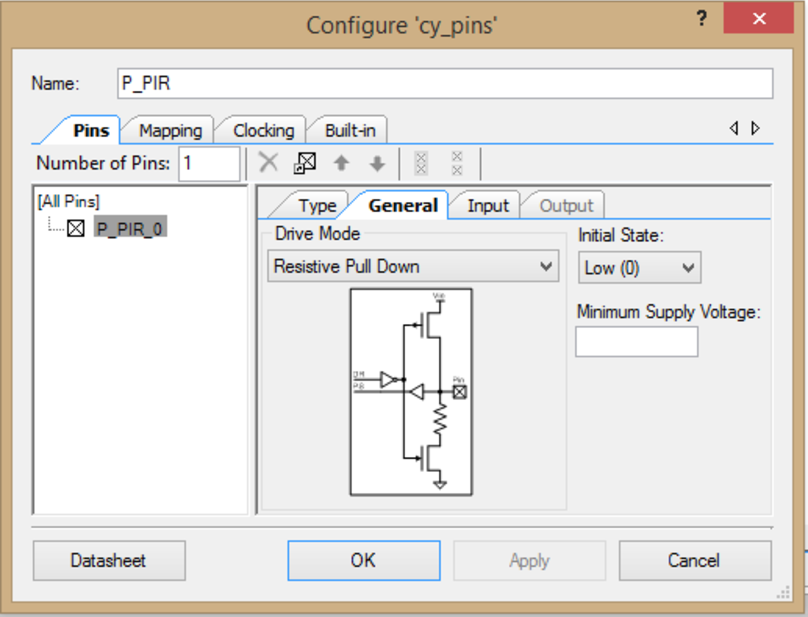
\includegraphics[width=0.60\textwidth]{filer/pics/pir_api_topdesign_2}}
\caption{Konfiguration af pir pin}
\label{lab:pir_topdesign_2}
\end{figure}


\subsubsection*{Source fil}
\begin{lstlisting}[language=C]
CY_ISR(P_PIR)
{  
    loadData_movementDetekt();   
}
\end{lstlisting}

\section{Software (BS JC)}
Efter sekvensdiagrammerne, klassediagrammet og klassebeskrivelser er designfasen afsluttet. Implementeringen starter så med at lave alle de forskellige klasser. Dette ender ud i de følgende statiske klassediagrammer.

Da vi har arbejdet i Qt frameworket til at oprette og styre vores user interface på Devkit8000 så har vi gjort brug af mange af deres klasser. F.eks anvendes der ofte en \verb+QString+ istedet for en \verb+std::string+. Der er design billeder der viser hvordan vores UI ser ud når det bliver deployed på Devkit8000. Design filerne er dem i UI klassen som starter med \verb+win+ som ses på figur \ref{fig:class_static_dev}. Disse UI billeder har nogle knapper som kan sende nogle signaler til vores funktioner, et såkaldt event system. Event systemet er det som bringer os rundt i UI'en ved at kalde nogle bestemte funktioner når de pågældende knapper bliver trykket på osv.

Selve strukturen er opbygget omkring objektet \verb+QStackedWindget winStack_+. Dette er et objekt i Qt frameworket som kan stacke billeder. Denne er altså en stak af alle de UI billeder som vi har i systemet. Når man skifter vindue, vælger man altså blot hvilket billede som ligger øverst i stakken, og på den måde bliver synligt. 

\subsection{Master (JC)}
%% SW klassediagram static

\begin{figure}[!htbp] \centering
{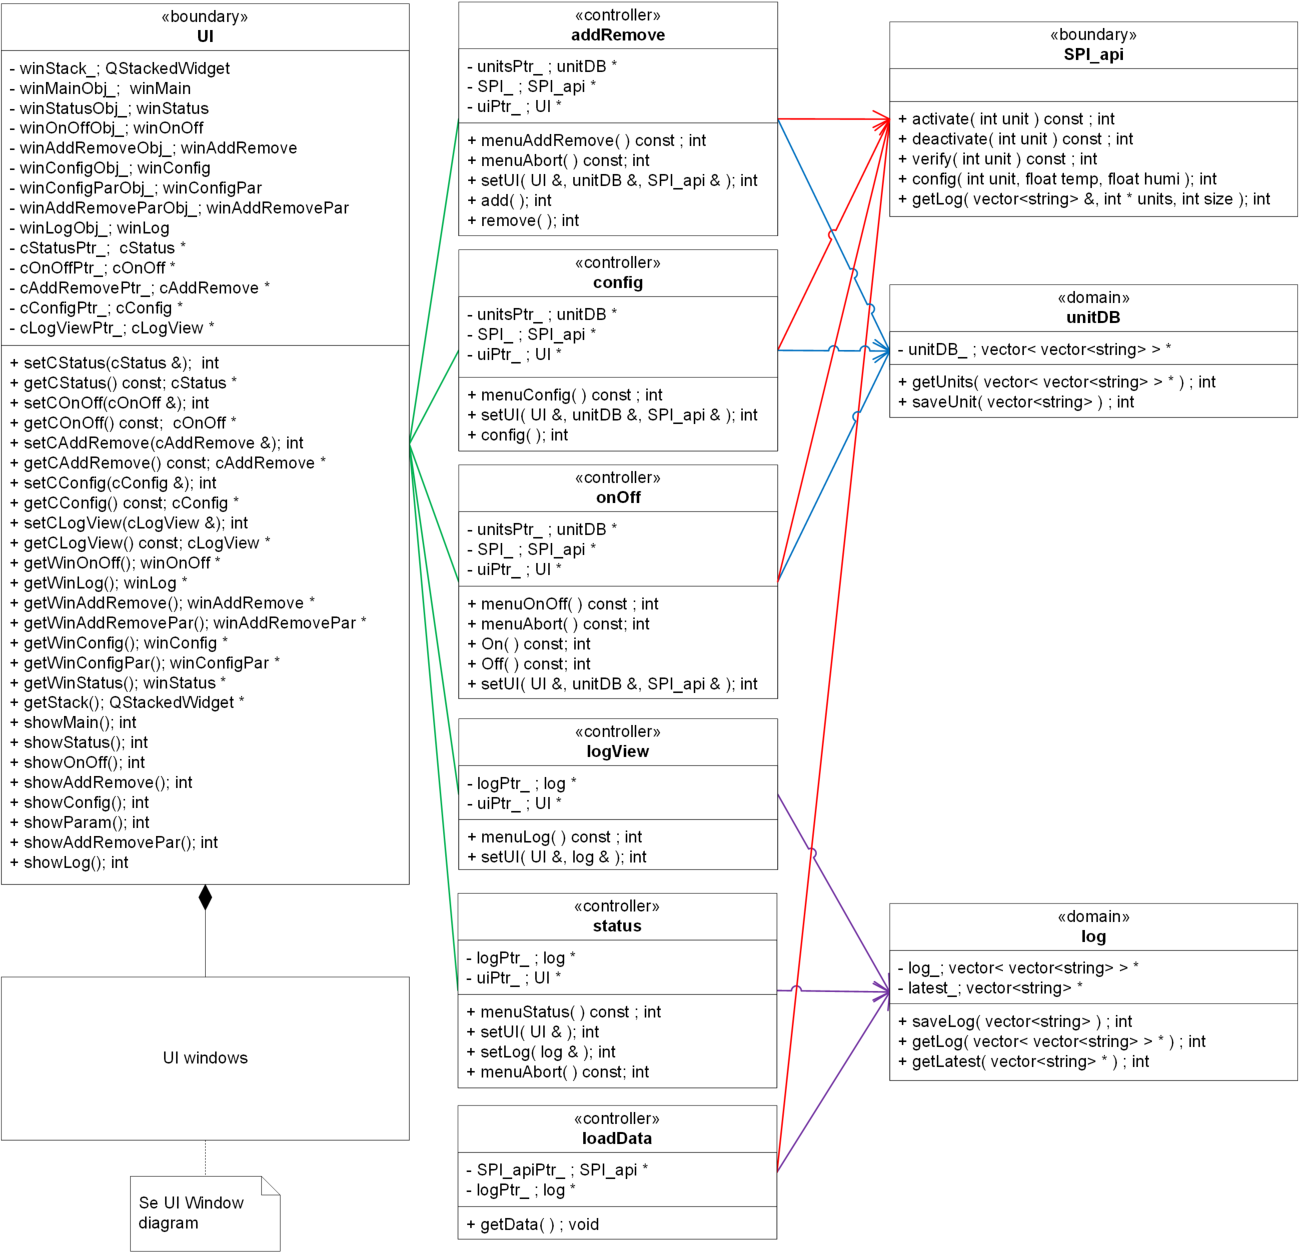
\includegraphics[scale=0.7]{filer/implementering/sw_class_devkit_static}}
\caption{Statisk klassediagram for Master (Devkit8000)}
\label{fig:class_static_dev}
\end{figure}

\begin{figure}[!htbp] \centering
{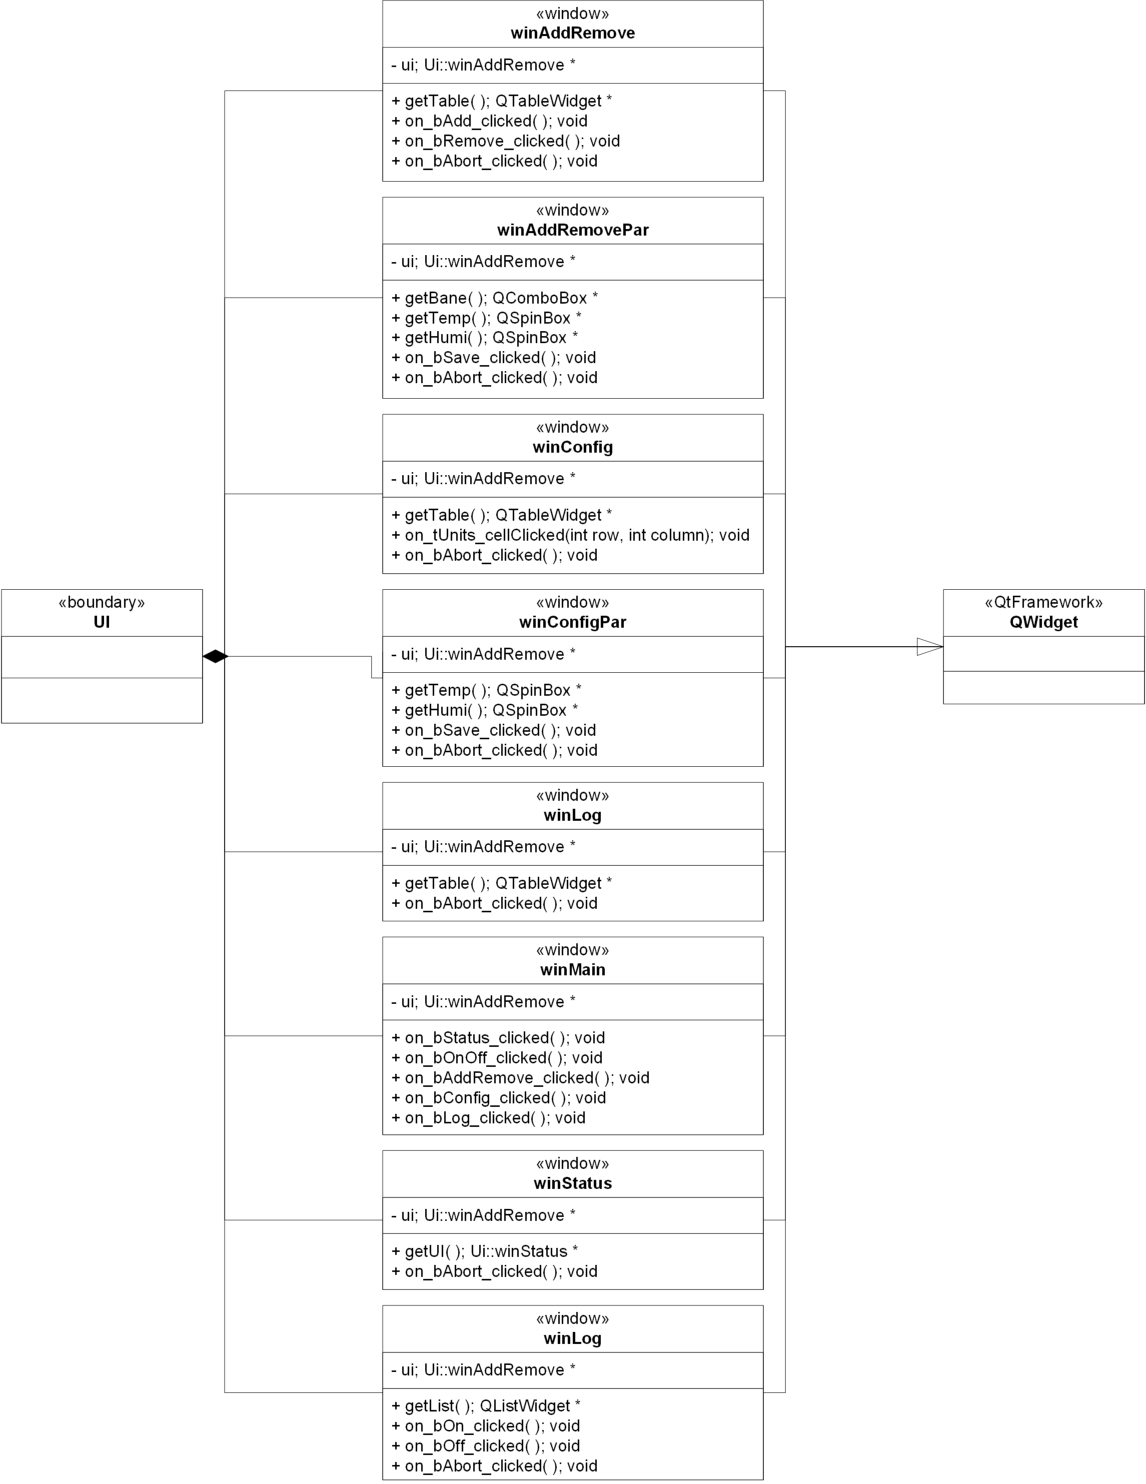
\includegraphics[scale=0.7]{filer/implementering/sw_class_devkit_windows_static}}
\caption{Statisk klassediagram for vinduer på Master (Devkit8000)}
\label{fig:class_static_dev_window}
\end{figure}


\clearpage

\subsection{Enhed (BS)}
%% SW klassediagram static

\begin{figure}[!htbp] \centering
{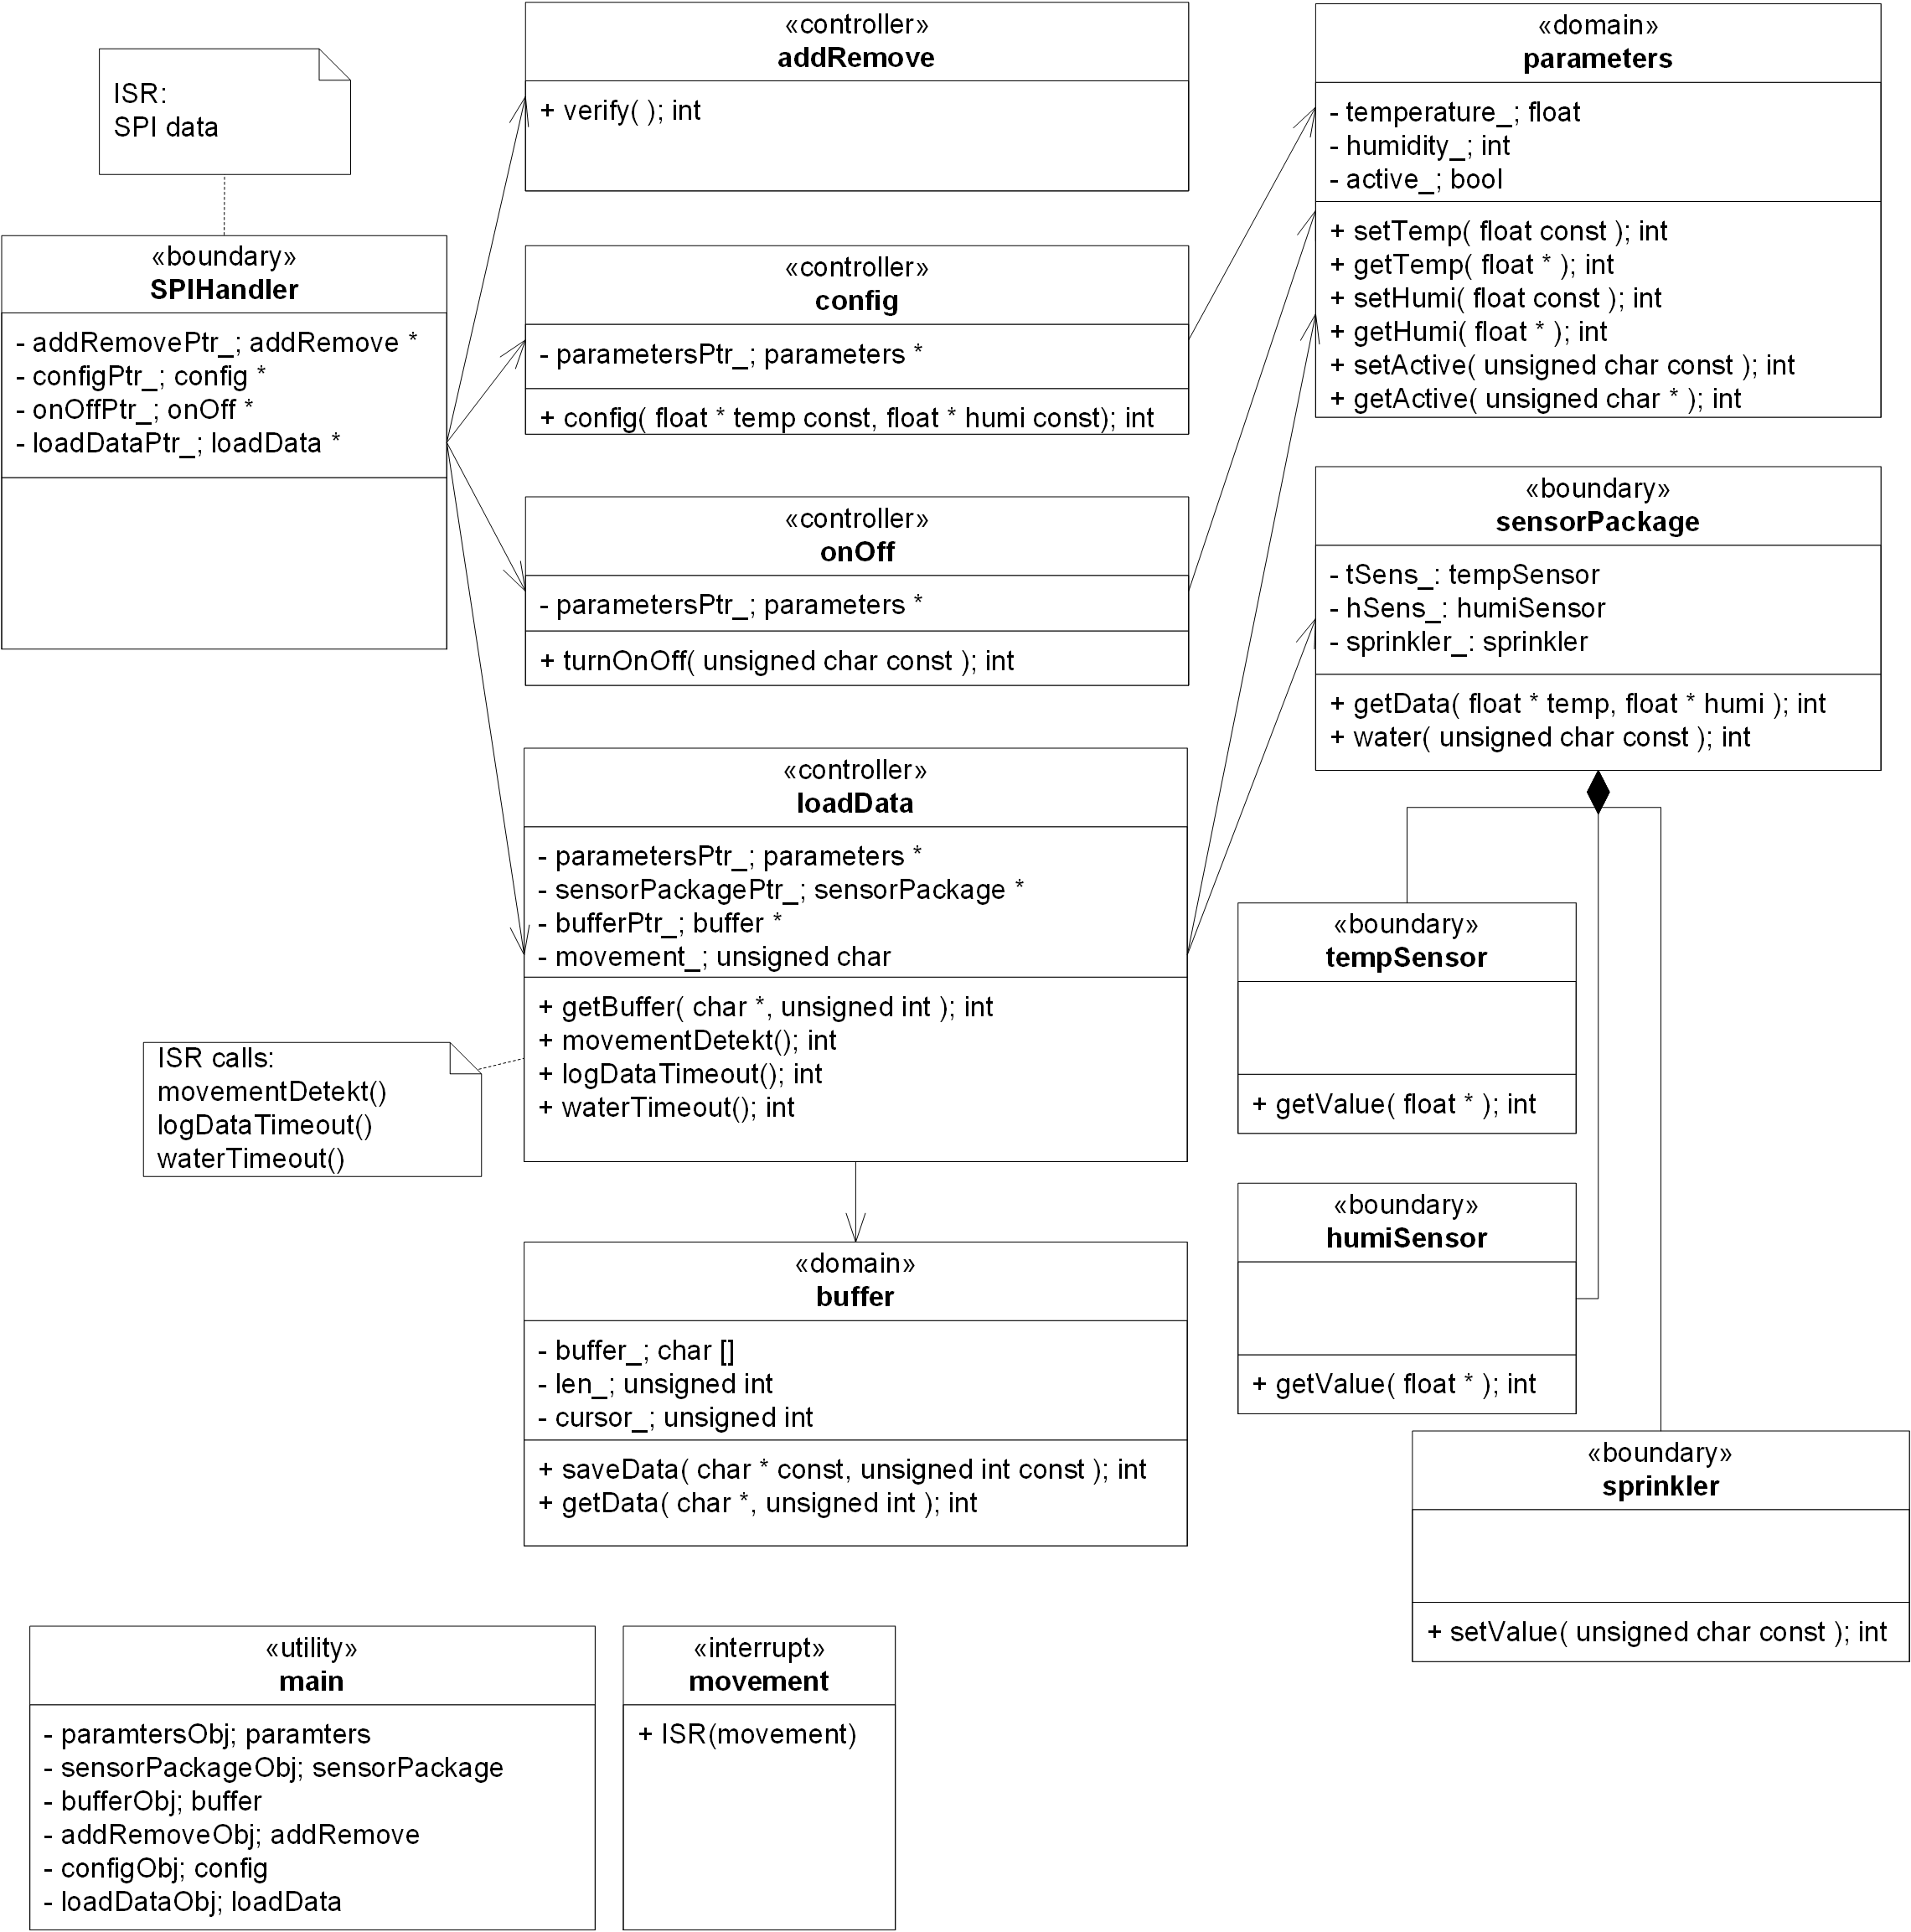
\includegraphics[scale=0.7]{filer/design/sw_class_psoc_static}}
\caption{Statisk klassediagram for Enhed (PSoC)}
\label{fig:class_psoc_static_dev}
\end{figure}



